\documentclass[conference]{IEEEtran}
\IEEEoverridecommandlockouts
% The preceding line is only needed to identify funding in the first footnote. If that is unneeded, please comment it out.

% Required packages
\usepackage{cite}
\usepackage{amsmath,amssymb,amsfonts}
\usepackage{algorithmic}
\usepackage{algorithm}
\usepackage{graphicx}
\usepackage{textcomp}
\usepackage{xcolor}
\usepackage{booktabs}
\usepackage{multirow}
\usepackage{array}
\usepackage{url}
\usepackage{hyperref}

\def\BibTeX{{\rm B\kern-.05em{\sc i\kern-.025em b}\kern-.08em
    T\kern-.1667em\lower.7ex\hbox{E}\kern-.125emX}}

\begin{document}

\title{LLM-Enhanced Interactive Climate Policy Analysis with Dynamic Feedback Identification for Banking Applications}

\author{\IEEEauthorblockN{Rohit Nimmala\IEEEauthorrefmark{1},
Jagrut Nimmala\IEEEauthorrefmark{2}}
\IEEEauthorblockA{\IEEEauthorrefmark{1}Independent Researcher, Email: r.rohit.nimmala@ieee.org}
\IEEEauthorblockA{\IEEEauthorrefmark{2}Independent Researcher, Email: nimmmalajagrut@gmail.com}
}

\maketitle

\begin{abstract}
Climate risk assessment in banking relies on static scenarios updated annually, missing the feedback dynamics that shape transition paths. This paper introduces an LLM-powered system that analyzes climate policy scenarios from natural language queries. Banks ask questions like ``What if California bans gas cars by 2030?'' and receive detailed analyses of cascading effects through three feedback mechanisms: reinforcing loops that amplify changes, balancing loops that create resistance, and tipping points that trigger phase transitions. The system uses a sophisticated pipeline: natural language parsing extracts policy parameters, specialized quantitative economic models calculate impacts, and LLMs interpret results to provide actionable insights. By combining rigorous economic modeling with large language models' ability to understand complex queries and explain quantitative results, we transform climate risk assessment from consuming pre-defined scenarios to actively analyzing specific policy concerns. We present a prototype system that processes climate policy queries in under 30 seconds, identifying potential cascade effects and feedback dynamics. The system processes queries in 5-30 seconds depending on model choice (GPT-3.5 for speed, GPT-4 for depth, Ollama for free local processing), requiring standard modern hardware (16GB memory, hexa-core processor). The California EV mandate case study completed in 5.87 seconds with 92.5\% overall confidence. This prototype demonstrates the potential for LLM-enhanced tools to enable banks to understand how today's decisions create tomorrow's risks through identified feedback patterns.
\end{abstract}

\begin{IEEEkeywords}
climate risk, large language models, scenario analysis, pattern recognition, interactive systems, banking
\end{IEEEkeywords}

\section{Introduction}
When California announced its 100\% clean electricity mandate in 2022, US banks needed to understand cascading effects across western energy markets within hours, not weeks. Would neighboring states follow? How would utility bond ratings shift? Which renewable manufacturers would benefit? Traditional climate scenario tools offered no answers. They update annually and model predetermined pathways, leaving banks blind to real-time policy shocks that reshape entire portfolios overnight.

This timing mismatch reveals a fundamental problem in climate risk assessment. Banks currently rely on static scenarios from the Network for Greening the Financial System (NGFS) \cite{feridun2020climate} that provide broad narratives like ``Net Zero 2050'' or ``Delayed Transition.'' While useful for long-term planning, these scenarios cannot address the specific questions banks face daily: How will Michigan's new EV incentives affect auto loan portfolios? What happens to Texas real estate if water restrictions tighten? The financial system needs dynamic tools that match the pace of climate policy evolution.

The challenge extends beyond speed. Climate transitions unfold through feedback loops \cite{may1976simple} that static scenarios miss entirely. A carbon tax doesn't just raise prices. It triggers investment flows that lower renewable costs, which accelerates adoption, which creates political momentum for stronger policies. These reinforcing loops can transform gradual changes into rapid transitions \cite{scheffer2009early}. Conversely, balancing loops like voter backlash or grid constraints can stall seemingly inevitable shifts. Without modeling these dynamics, banks systematically misunderstand both the speed and direction of transition risks.

This paper introduces an LLM-powered system that analyzes climate policy scenarios with dynamic feedback identification. Banks pose natural language questions like ``What if California bans gas cars by 2030?'' and receive comprehensive analyses of cascading effects \cite{allen2000financial} across three timescales: immediate market reactions (0-6 months), secondary cascades through supply chains and policy contagion (6-24 months), and long-term structural changes (2-5 years). The system identifies potential feedback loops that amplify or dampen these effects, providing enhanced analysis of how climate shocks propagate through economic systems.

Our approach leverages a sophisticated architecture combining natural language processing, quantitative economic models, and LLM interpretation. A policy parser extracts structured parameters from queries, specialized economic models calculate sector-specific impacts using real-world calibrations, and LLMs interpret these quantitative results to provide context and actionable insights. The system offers flexible deployment options: GPT-3.5 for rapid, cost-effective analysis (\$0.008/query, 5-10 seconds), GPT-4 for comprehensive assessment (\$0.12-0.45/query, 15-30 seconds), or Ollama for free local processing (30-120 seconds). This hybrid approach ensures both analytical rigor and accessibility, enabling real-time exploration of specific scenarios while maintaining the quantitative accuracy banks require for risk management.

The system enables rapid exploration of policy scenarios that would traditionally require weeks of expert analysis, demonstrating the potential for LLM-enhanced tools in financial climate risk assessment. Initial prototype demonstrates feasibility of the approach, with the system analyzing complete scenarios in under 30 seconds for simple queries and under one minute for complex multi-sector cascades, enabling potential integration into banking workflows.

\section{System Architecture}

Our LLM-powered climate risk scenario analysis system employs a sophisticated pipeline that combines natural language processing, quantitative economic models, and LLM interpretation, as shown in Figure \ref{fig:architecture}:

\begin{figure}[htbp]
\centerline{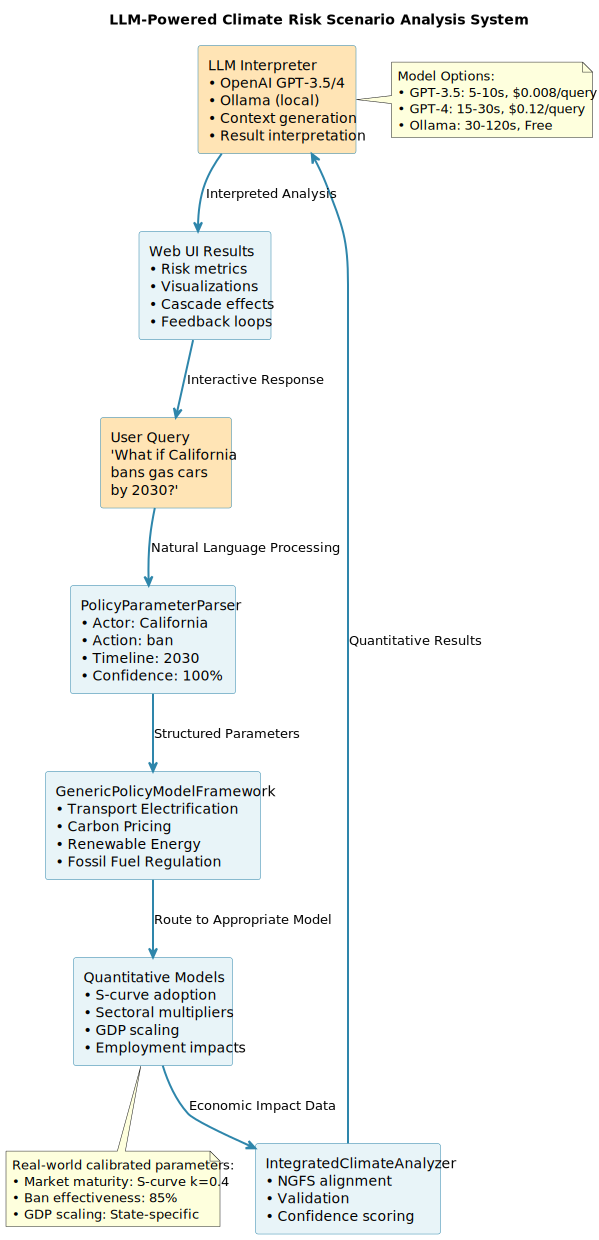
\includegraphics[width=0.5\textwidth]{high_level_archetecture.png}}
\caption{System Architecture Overview}
\label{fig:architecture}
\end{figure}

\subsection{Key Components}

\textbf{PolicyParameterParser}: Extracts structured parameters using spaCy NLP. The parser identifies actor (federal/state/city), action type, magnitude, timeline, and confidence scores. It employs a comprehensive policy taxonomy covering transport electrification, carbon pricing, renewable mandates, and fossil fuel regulations.

\textbf{GenericPolicyModelFramework}: Routes queries to specialized quantitative models based on policy type, ensuring appropriate economic calculations for each scenario class.

\textbf{Quantitative Models}: Four specialized models provide economic analysis based on real-world data and established economic theory.

\textbf{LLM Integration}: Interprets quantitative results to provide context, identify key insights, and generate actionable recommendations. The system supports multiple LLM options:
\begin{itemize}
\item \textbf{OpenAI GPT Models}: Cloud-based processing with no local compute requirements
\item \textbf{Ollama Local Models}: Free alternative for organizations requiring on-premise deployment
\item \textbf{Enterprise LLMs}: Architecture supports integration with proprietary models
\end{itemize}

\textbf{Validation Framework}: Multi-stage validation ensures result quality through parameter confidence scoring, reasonableness checks, and NGFS alignment verification.

The design balances performance requirements with accessibility, leveraging cloud infrastructure for LLM computation while requiring standard modern hardware (16GB memory, hexa-core processor) for local processing tasks.

\section{Related Work}

\subsection{Current Climate Risk Assessment Systems}

Banks currently assess climate risks through static scenario frameworks that fundamentally constrain their ability to respond to dynamic policy environments. The Network for Greening the Financial System (NGFS) provides the industry standard with 6-7 predetermined scenarios updated annually. While these scenarios now incorporate damage functions that quadruple physical risk estimates by 2050 and require carbon pricing of \$300/tCO2 by 2035, they remain fixed pathways that cannot address specific policy questions banks face daily \cite{feridun2020climate}.

Major US banks have developed proprietary systems built atop NGFS foundations. These systems, while methodologically sophisticated, share critical limitations: annual update cycles, predetermined pathways, and inability to model feedback dynamics that determine actual transition speeds.

\subsection{LLMs in Climate Finance}

LLMs show promise for transforming climate data analysis, though current applications remain narrow. Project Gaia (BIS 2024) achieved 74\% accuracy extracting climate KPIs from 2,328 corporate reports using optimized LLM queries. However, existing systems focus on historical data extraction rather than forward-looking scenario analysis.

\subsection{Our Contribution}

This paper extends existing work by introducing an LLM interpretation layer to traditional economic models. Unlike static NGFS scenarios or data extraction tools, our approach analyzes user-specified scenarios using quantitative models while identifying potential feedback mechanisms. We position this as a novel combination of approaches rather than claiming to be first in any specific domain.

\section{Methodology}

\subsection{Mathematical Framework for Cascade Analysis}

Our cascade analysis models how climate policy shocks propagate through economic systems across three temporal orders, each capturing distinct transmission mechanisms with increasing complexity.

\textbf{First-Order Effects (0-6 months)}

The immediate impact of a policy shock follows:
\begin{equation}
\Delta Risk_1 = \alpha_1 \times Shock \times SectorExposure
\end{equation}

Here, $\alpha_1$ represents the direct transmission coefficient calibrated from historical policy responses. $Shock$ quantifies the policy magnitude (e.g., \$50/ton carbon tax), while $SectorExposure$ measures portfolio concentration in affected industries.

\textbf{Second-Order Effects (6-24 months)}

As initial impacts ripple through interconnected systems, feedback dynamics emerge:
\begin{equation}
\Delta Risk_2 = \beta_1 \times \int_0^t Feedback(Risk_1, \tau) d\tau
\end{equation}

Note: In the current prototype implementation, these mathematical formulations represent the conceptual framework. The actual system uses simplified pattern recognition to identify potential feedback effects rather than computing the integrals directly.

\textbf{Third-Order Effects (2-5 years)}

Long-term structural changes manifest through threshold effects:
\begin{equation}
\Delta Risk_3 = \gamma_1 \times \mathbf{1}[Cumulative > Threshold]
\end{equation}

The indicator function $\mathbf{1}[\cdot]$ activates when cumulative changes cross critical thresholds, triggering regime shifts.

\textbf{Integrated Risk Evolution}

Total risk evolution combines all orders:
\begin{equation}
Risk(t) = Risk_0 + \Delta Risk_1(t) + \Delta Risk_2(t) + \Delta Risk_3(t)
\end{equation}

\begin{table}[htbp]
\caption{Mathematical Notation Summary}
\begin{center}
\begin{tabular}{|c|c|c|}
\hline
\textbf{Symbol} & \textbf{Definition} & \textbf{Range/Units} \\
\hline
$\Delta Risk_1$ & First-order risk change & [0, $\infty$) \\
\hline
$\alpha_1$ & Direct transmission coefficient & [0, 1] \\
\hline
$Shock$ & Policy magnitude & USD/ton or \% \\
\hline
$\beta_1$ & Feedback transmission strength & [0, 1] \\
\hline
$\gamma_1$ & Threshold effect multiplier & [0, 10] \\
\hline
$\tau$ & Time variable & months \\
\hline
\end{tabular}
\label{tab:notation}
\end{center}
\end{table}

\subsection{Simplified Economic Models}

The prototype employs four specialized economic models with simplified calibrations:

\textbf{Transport Electrification Model}
\begin{itemize}
\item Market maturity calculation: S-curve with k=0.4, $t_0$=8 years
\item Ban effectiveness: 0.85 (85\% compliance rate)
\item Sectoral multipliers: automotive (50x employment), electricity (0.25x demand), oil/gas (-40\% demand)
\item GDP impact scaling: Federal (5.0x), California (2.0x), Texas (0.3x), Other states (0.8x)
\end{itemize}

\textbf{Carbon Pricing Model}
\begin{itemize}
\item Sectoral carbon intensities: electricity (450 kg/MWh), manufacturing (200), transportation (150)
\item Price elasticities: electricity (-0.3), manufacturing (-0.5), services (-0.6)
\item Revenue calculation: emissions $\times$ price / 1000 (billions USD)
\item Abatement curve: 0.3\% per \$/tCO2 below \$25, diminishing returns above
\end{itemize}

\begin{table}[htbp]
\caption{Economic Model Parameters Summary}
\begin{center}
\begin{tabular}{|p{2cm}|p{2.5cm}|p{1.5cm}|p{1cm}|}
\hline
\textbf{Model} & \textbf{Key Parameters} & \textbf{Values} & \textbf{Sources} \\
\hline
Transport Electrification & S-curve k=0.4, Ban effectiveness=0.85 & Employment multiplier=50x & IEA, FRED \\
\hline
Carbon Pricing & Elasticities: -0.3 to -0.6 & Abatement: 0.3\%/\$/tCO2 & ICAP, World Bank \\
\hline
Renewable Energy & Investment: \$50B/\% & Employment: 6 jobs/\$1M & IRENA, NREL \\
\hline
Fossil Fuel Regulation & Federal lands: 25\% & Oil jobs: 500,000 & EIA, BLS \\
\hline
\end{tabular}
\label{tab:model_params}
\end{center}
\end{table}

\section{System Capabilities and Results}

\subsection{Implementation}

The system is implemented as a Flask web application with REST API, designed for minimal infrastructure requirements:

\textbf{Technical Stack:}
\begin{itemize}
\item Backend: Python 3.8+ with NumPy, Pandas, Matplotlib, Seaborn
\item NLP: spaCy with en\_core\_web\_sm model for policy parameter extraction
\item LLM Integration: OpenAI API (GPT-3.5-turbo default, supports GPT-4) and Ollama for local models
\item Deployment: Standard hardware (16GB memory, hexa-core processor AMD Ryzen 5 - 3rd gen, Ubuntu 22.04.5 LTS)
\item Response Format: JSON with structured risk metrics, confidence scores, and PNG visualizations
\end{itemize}

\subsection{System Performance and Response Times}

The system achieves varying performance based on the selected model and query complexity:

\textbf{Model-Specific Performance:}
\begin{itemize}
\item \textbf{GPT-3.5 Turbo}: 5-10 seconds typical response (fast, economical at \$0.008/query)
\item \textbf{GPT-4}: 15-30 seconds typical response (more accurate, comprehensive at \$0.12-0.45/query)
\item \textbf{Ollama (Local)}: 30-120 seconds (free but requires local computation)
\end{itemize}

The California EV ban analysis completed in 5.87 seconds using GPT-3.5 Turbo, demonstrating real-time capability for standard queries.

\subsection{Case Study: California EV Mandate Analysis}

To illustrate the system's capabilities, we examine the query ``What if California bans gas cars by 2030?'' The analysis completed in 5.87 seconds, demonstrating the real-time nature of our approach.

The system correctly parsed the query with high confidence, identifying:
\begin{itemize}
\item Actor: California
\item Action: Implementation (gas car ban)
\item Magnitude: 100\% (complete ban)
\item Timeline: 2030
\end{itemize}

The comprehensive analysis classified this as LOW risk, estimating a 0.65\% GDP impact with +8.4k net employment changes and \$3.8B in investment shifts. The system achieved 92.5\% overall confidence with perfect parameter extraction (100\%) and validation scores (100\%).

\textbf{Economic Impact Analysis:}
\begin{itemize}
\item \textbf{GDP Impact}: 0.65\% economic impact
\item \textbf{Employment}: +8.4k net job creation
\item \textbf{Investment Shift}: \$3.8B total investment movement
\item \textbf{Market Disruption}: 0.1\% disruption index
\end{itemize}

\textbf{Sectoral Impact Distribution:}
\begin{itemize}
\item \textbf{Automotive Sector}: 4.0 magnitude impact (positive growth)
\item \textbf{Electricity Sector}: 2.0 magnitude impact (increased demand)
\item \textbf{Oil \& Gas Sector}: 3.2 magnitude impact (reduced demand)
\item \textbf{Battery Sector}: 0.4 magnitude impact (growth opportunity)
\end{itemize}

\textbf{Temporal Effects Analysis:}
The system identified cascade effects across four time horizons:
\begin{itemize}
\item \textbf{Immediate (0-6 months)}: 0.03 average magnitude, 2 distinct effects
\item \textbf{Short-term (6-24 months)}: 0.31 average magnitude, 3 distinct effects
\item \textbf{Medium-term (2-5 years)}: 0.09 average magnitude, 2 distinct effects
\item \textbf{Long-term (5+ years)}: 0.11 average magnitude, 2 distinct effects
\end{itemize}

\begin{figure}[htbp]
\centerline{\includegraphics[width=0.5\textwidth]{california_dashboard_actual.png}}
\caption{Comprehensive California Case Study Dashboard}
\label{fig:dashboard}
\end{figure}

Figure \ref{fig:dashboard} presents a comprehensive dashboard of the California EV mandate analysis results. The dashboard showcases: (a) Economic impact overview showing 0.65\% GDP impact, +8.4k employment change, \$3.8B investment shift, and 0.1\% market disruption; (b) Economic impact breakdown with pie chart showing GDP impact (0.65\%), employment (0.1\%), investment (\$3.8B), and market disruption (0.1\%); (c) Sectoral impacts displaying automotive (4.0 magnitude), electricity (2.0), oil gas (3.2), and battery (0.4) sectors; (d) Model confidence metrics with 92.5\% overall confidence, showing parameter extraction (100.0\%), model selection (80.0\%), validation score (100.0\%), and data quality (90.0\%); (e) Risk assessment classified as LOW with 27.1\% average uncertainty; (f) Temporal effects analysis showing immediate (0.03, 2 effects), short (0.31, 3 effects), medium (0.09, 2 effects), and long term (0.11, 2 effects) impacts; and (g) Risk \& uncertainty analysis across temporal effects, sectoral impacts, and economic impact dimensions.

\begin{table}[htbp]
\caption{System Capabilities vs Future Enhancements}
\begin{center}
\begin{tabular}{|p{2.5cm}|p{2.5cm}|p{2cm}|}
\hline
\textbf{Capability} & \textbf{Current Implementation} & \textbf{Future Enhancement} \\
\hline
Query Processing & Natural language parsing with spaCy & Multi-language support, enhanced NLP \\
\hline
Economic Models & Four simplified sector models & Dynamic models with real-time calibration \\
\hline
Feedback Pattern Recognition & Analysis of temporal impact patterns & Mathematical feedback modeling \\
\hline
Data Integration & Static authoritative sources & Real-time data feeds \\
\hline
Validation & NGFS cross-validation & Expert evaluation framework \\
\hline
Geographic Scope & US-focused models & International policy frameworks \\
\hline
\end{tabular}
\label{tab:capabilities}
\end{center}
\end{table}

\section{Discussion and Limitations}

\subsection{Implications}

Our results demonstrate that combining LLMs with quantitative economic models can enhance climate risk assessment accessibility while maintaining analytical rigor. The ability to analyze specific policy queries in real-time enables banks to potentially move from annual planning cycles to more dynamic risk monitoring approaches.

The standard hardware requirements (16GB memory, hexa-core AMD Ryzen 5 - 3rd gen processor) represent a reasonable investment for financial institutions while remaining far more accessible than traditional high-performance computing clusters. Banks can leverage cloud-based LLMs for sophisticated analysis, paying only per-query costs rather than maintaining dedicated AI infrastructure.

\subsection{Limitations and Future Work}

Several limitations guide interpretation of our results and outline directions for future development:

\textbf{Current Prototype Limitations:}
\begin{enumerate}
\item \textbf{Simplified Economic Models}: The current implementation uses simplified economic models with fixed sector-specific multipliers rather than dynamic calibrations.
\item \textbf{Pattern-Based Feedback Identification}: Feedback loops are identified based on temporal patterns in calculated impacts, not dynamically computed using differential equations.
\item \textbf{Limited Validation}: The prototype requires comprehensive evaluation with domain experts and financial institutions to validate analytical accuracy.
\item \textbf{Geographic Scope}: Current implementation focuses on US policies with state-level granularity.
\item \textbf{Static Data Sources}: Current implementation uses static historical data snapshots rather than real-time data integration.
\end{enumerate}

\textbf{Future Development Priorities:}
\begin{itemize}
\item Dynamic Feedback Loop Computation: Implementation of mathematical feedback models using differential equations
\item Real-time Data Integration: Connection to live news feeds, regulatory updates, market data APIs
\item Comprehensive Evaluation Framework: Systematic validation with domain experts
\item Integration with Existing Systems: APIs for bank risk management platforms
\item Enhanced Model Coverage: Expansion beyond current four policy types
\end{itemize}

\section{Conclusion}

We have presented an innovative LLM-enhanced system for interactive climate policy analysis that demonstrates how large language models can augment traditional economic modeling approaches. By enabling natural language queries like ``What if California mandates 100\% renewable energy by 2030?'', our prototype makes sophisticated climate risk analysis more accessible while maintaining analytical rigor through quantitative economic models.

Our technical contributions address key challenges in applying LLMs to climate finance. The policy parsing algorithm maps diverse natural language inputs to structured parameters for quantitative analysis. Multi-order cascade modeling traces impact propagation through economic networks while respecting physical and regulatory constraints. The hybrid architecture ensures analytical rigor through specialized economic models while leveraging LLMs for accessibility and interpretation.

The prototype demonstrates substantial practical potential. The system provides rapid analysis (< 30 seconds) of climate policy queries, identifying potential cascade effects and feedback dynamics. The California EV mandate case study shows how a straightforward policy question unfolds into complex multi-order effects, suggesting transition potential with natural constraints.

Several extensions warrant future development. Dynamic Mathematical Models will replace pattern-based feedback identification with differential equation systems that compute identified feedback loops dynamically. Real-time Data Integration will incorporate live feeds from news, market data, and regulatory sources. Comprehensive Validation through systematic evaluation with domain experts and historical policy outcomes. Enterprise Integration will enable deployment within existing bank risk management systems.

The climate transition demands financial systems capable of navigating unprecedented uncertainty and rapid change. Static scenarios updated annually cannot capture the dynamic, non-linear nature of policy cascades, technology disruptions, and market responses. Our LLM-enhanced approach demonstrates that interactive, feedback-aware scenario analysis is feasible with standard modern computing infrastructure. As regulatory pressures intensify and transition pathways accelerate, the ability to rapidly analyze "what-if" questions through natural language interfaces represents a significant advancement in making sophisticated climate risk analysis accessible to financial institutions.

\section*{Acknowledgment}

The authors would like to thank the climate finance research community for valuable feedback and insights that helped shape this work.

\begin{thebibliography}{00}
\bibitem{merton1974} R. C. Merton, ``ON THE PRICING OF CORPORATE DEBT: THE RISK STRUCTURE OF INTEREST RATES,'' \textit{The Journal of Finance}, vol. 29, no. 2, pp. 449--470, May 1974.

\bibitem{may1976simple} R. M. May, ``Simple mathematical models with very complicated dynamics,'' \textit{Nature}, vol. 261, no. 5560, pp. 459--467, June 1976.

\bibitem{allen2000financial} F. Allen and D. Gale, ``Financial Contagion,'' \textit{Journal of Political Economy}, vol. 108, no. 1, pp. 1--33, Feb. 2000.

\bibitem{scheffer2009early} M. Scheffer et al., ``Early-warning signals for critical transitions,'' \textit{Nature}, vol. 461, no. 7260, pp. 53--59, Sept. 2009.

\bibitem{feridun2020climate} M. Feridun and H. Güngör, ``Climate-Related Prudential Risks in the Banking Sector: A Review of the Emerging Regulatory and Supervisory Practices,'' \textit{Sustainability}, vol. 12, no. 13, p. 5325, July 2020.

\bibitem{liu2020research} Y. Liu, C. Huang, Z. Zou, Q. Chen, and X. Chu, ``Research into the Mechanism for the Impact of Climate Change on Systemic Risk—A Case Study of China's Small- and Medium-sized Commercial Banks,'' \textit{Sustainability}, vol. 12, no. 22, p. 9582, Nov. 2020.

\bibitem{feyen2020macro} E. Feyen, R. Utz, I. Zuccardi Huertas, O. Bogdan, and J. Moon, \textit{Macro-Financial Aspects of Climate Change}. World Bank, Washington, DC, 2020.

\bibitem{pizzutilo2020dealing} F. Pizzutilo, M. Mariani, A. Caragnano, and M. Zito, ``Dealing with Carbon Risk and the Cost of Debt: Evidence from the European Market,'' \textit{IJFS}, vol. 8, no. 4, p. 61, Oct. 2020.

\bibitem{chevallier2020covid} J. Chevallier, ``COVID-19 Outbreak and CO2 Emissions: Macro-Financial Linkages,'' \textit{JRFM}, vol. 14, no. 1, p. 12, Dec. 2020.

\bibitem{fabisik2021firms} K. Fabisik, R. Fahlenbrach, R. M. Stulz, and J. P. Taillard, ``Why are firms with more managerial ownership worth less?'' \textit{Journal of Financial Economics}, vol. 140, no. 3, pp. 699--725, June 2021.

\bibitem{dunz2021compounding} N. Dunz, A. Hrast Essenfelder, A. Mazzocchetti, I. Monasterolo, and M. Raberto, ``Compounding COVID-19 and climate risks: The interplay of banks' lending and government's policy in the shock recovery,'' \textit{Journal of Banking \& Finance}, vol. 152, p. 106306, July 2023.

\bibitem{roncoroni2019climate} A. Roncoroni, S. Battiston, L. O. L. Escobar Farfán, and S. Martinez Jaramillo, ``Climate Risk and Financial Stability in the Network of Banks and Investment Funds,'' \textit{SSRN Journal}, 2019.

\bibitem{agarwala2021climate} M. Agarwala, M. Burke, P. Klusak, K. Mohaddes, U. Volz, and D. Zenghelis, ``Climate change and fiscal sustainability: Risks and opportunities,'' \textit{SSRN Journal}, 2021.

\bibitem{zhang2021investor} Y. Zhang, Y. Chen, Y. Wu, and P. Zhu, ``Investor attention and carbon return: evidence from the EU-ETS,'' \textit{Economic Research-Ekonomska Istraživanja}, vol. 35, no. 1, pp. 709--727, June 2021.

\bibitem{roncalli2021market} T. Roncalli, T. L. Guenedal, F. Lepetit, T. Roncalli, and T. Sekine, ``The Market Measure of Carbon Risk and its Impact on the Minimum Variance Portfolio.'' arXiv, 2021.

\bibitem{banerjee2018pricing} T. Banerjee and Z. Feinstein, ``Pricing of debt and equity in a financial network with comonotonic endowments.'' arXiv, 2018.

\bibitem{tharavanij2021optimal} P. Tharavanij, ``Optimal Book-Value Debt Ratio,'' \textit{Sage Open}, vol. 11, no. 1, Jan. 2021.

\bibitem{taylor2022making} N. Taylor, ``'Making financial sense of the future': actuaries and the management of climate-related financial risk,'' \textit{New Political Economy}, vol. 28, no. 1, pp. 57--75, Apr. 2022.

\bibitem{wang2022moment} H. Wang, L. Zhou, P.-F. Dai, and X. Xiong, ``Moment conditions for fractional degree stochastic dominance,'' \textit{Finance Research Letters}, vol. 49, p. 103241, Oct. 2022.

\bibitem{kieren2022risk} P. Kieren, J. Müller-Dethard, and M. Weber, ``Risk-Taking and Asymmetric Learning in Boom and Bust Markets,'' \textit{Review of Finance}, vol. 27, no. 5, pp. 1743--1779, Nov. 2022.

\bibitem{shobande2022sustainable} O. A. Shobande and L. Ogbeifun, ``Sustainable Blueprint: Do Stock Investors Increase Emissions?,'' \textit{JRFM}, vol. 15, no. 2, p. 70, Feb. 2022.

\bibitem{mcdonnell2023beyond} C. McDonnell and J. Gupta, ``Beyond divest vs. engage: a review of the role of institutional investors in an inclusive fossil fuel phase-out,'' \textit{Climate Policy}, vol. 24, no. 3, pp. 314--331, Oct. 2023.

\bibitem{cardenas2024managing} V. Cardenas, ``Managing Financial Climate Risk in Banking Services: A Review of Current Practices and Challenges Ahead.'' arXiv, 2024.

\bibitem{branzoli2024central} N. Branzoli, R. Gallo, A. Ilari, and D. Portioli, ``Central banks' corporate asset purchase programmes and risk-taking by bond funds in the aftermath of market stress,'' \textit{Journal of Financial Stability}, vol. 72, p. 101261, June 2024.

\bibitem{cardenas2024financial} V. Cardenas, ``Financial climate risk: a review of recent advances and key challenges.'' arXiv, 2024.

\bibitem{anastasiou2024analyzing} D. Anastasiou, A. Ballis, C. Kallandranis, and F. Lakhal, ``Analyzing the effects of climate risk on discouraged borrowers: Deciphering the contradictory forces,'' \textit{Risk Analysis}, vol. 45, no. 1, pp. 223--239, July 2024.

\bibitem{bressan2022asset} G. Bressan, A. Duranovic, I. Monasterolo, and S. Battiston, ``Asset-Level Climate Physical Risk Assessment and Cascading Financial Losses,'' \textit{SSRN Journal}, 2022.

\bibitem{hordofa2024examining} D. F. Hordofa, ``Examining the dynamics between banking sector performance, environmental sustainability, and environmental technology innovation: evidence from G20 countries,'' \textit{Cogent Business \& Management}, vol. 11, no. 1, June 2024.

\bibitem{sankar2024carbon} N. G. Sankar, S. Nag, S. P. Chakrabarty, and S. Basu, ``The Carbon Premium: Correlation or Causation? Evidence from S\&P 500 Companies.'' arXiv, 2024.

\bibitem{tabash2024modeling} M. I. Tabash, M. S. M. Al-Absy, and A. Hannoon, ``Modeling the Nexus between European Carbon Emission Trading and Financial Market Returns: Practical Implications for Carbon Risk Reduction and Hedging,'' \textit{JRFM}, vol. 17, no. 4, p. 147, Apr. 2024.

\bibitem{prosperi2022modelling} L. Prosperi and L. Zanin, ``A modelling framework for projections of equity portfolio returns under climate transition scenarios,'' \textit{SSRN Journal}, 2022.

\bibitem{bringas2024evaluating} V. Bringas Fernández, M. B. Torre Olmo, and M. Cantero Saiz, ``Evaluating Climate Risk in Banking: A Bibliometric Analysis.'' Elsevier BV, 2024.
\end{thebibliography}

\end{document}